\chapter{Anatomy of a Star-Shaped Thing} 
\label{sec:listing_pattern}
\lstset{style=6502Style}

If you look at Psychedelia at work for even a short time it is possible to guess at the fundamentals
of its operation. It takes the position of the cursor, paints a pattern with the cursor as its centre,
and then cycles each pixel it has painted through a series of colors.

As we look some more we might notice that the color a pixel changes to depends on what color it has already.
This becomes more noticable as we move the cursor around. If we're paying very close attention we might notice
that the number of avilable colors is fairly limited, perhaps as low as 7 or 8.

To improve our understanding any further we will need to look at the code. We might have to take this part slowly.
Although the code is very compact it might be hard to disentangle. Scanning through the 800 or so lines of assembly
we notice something relevant to our interests:

\clearpage
\begin{figure}[H]
    \centering
    \begin{adjustbox}{width=12cm,center}
      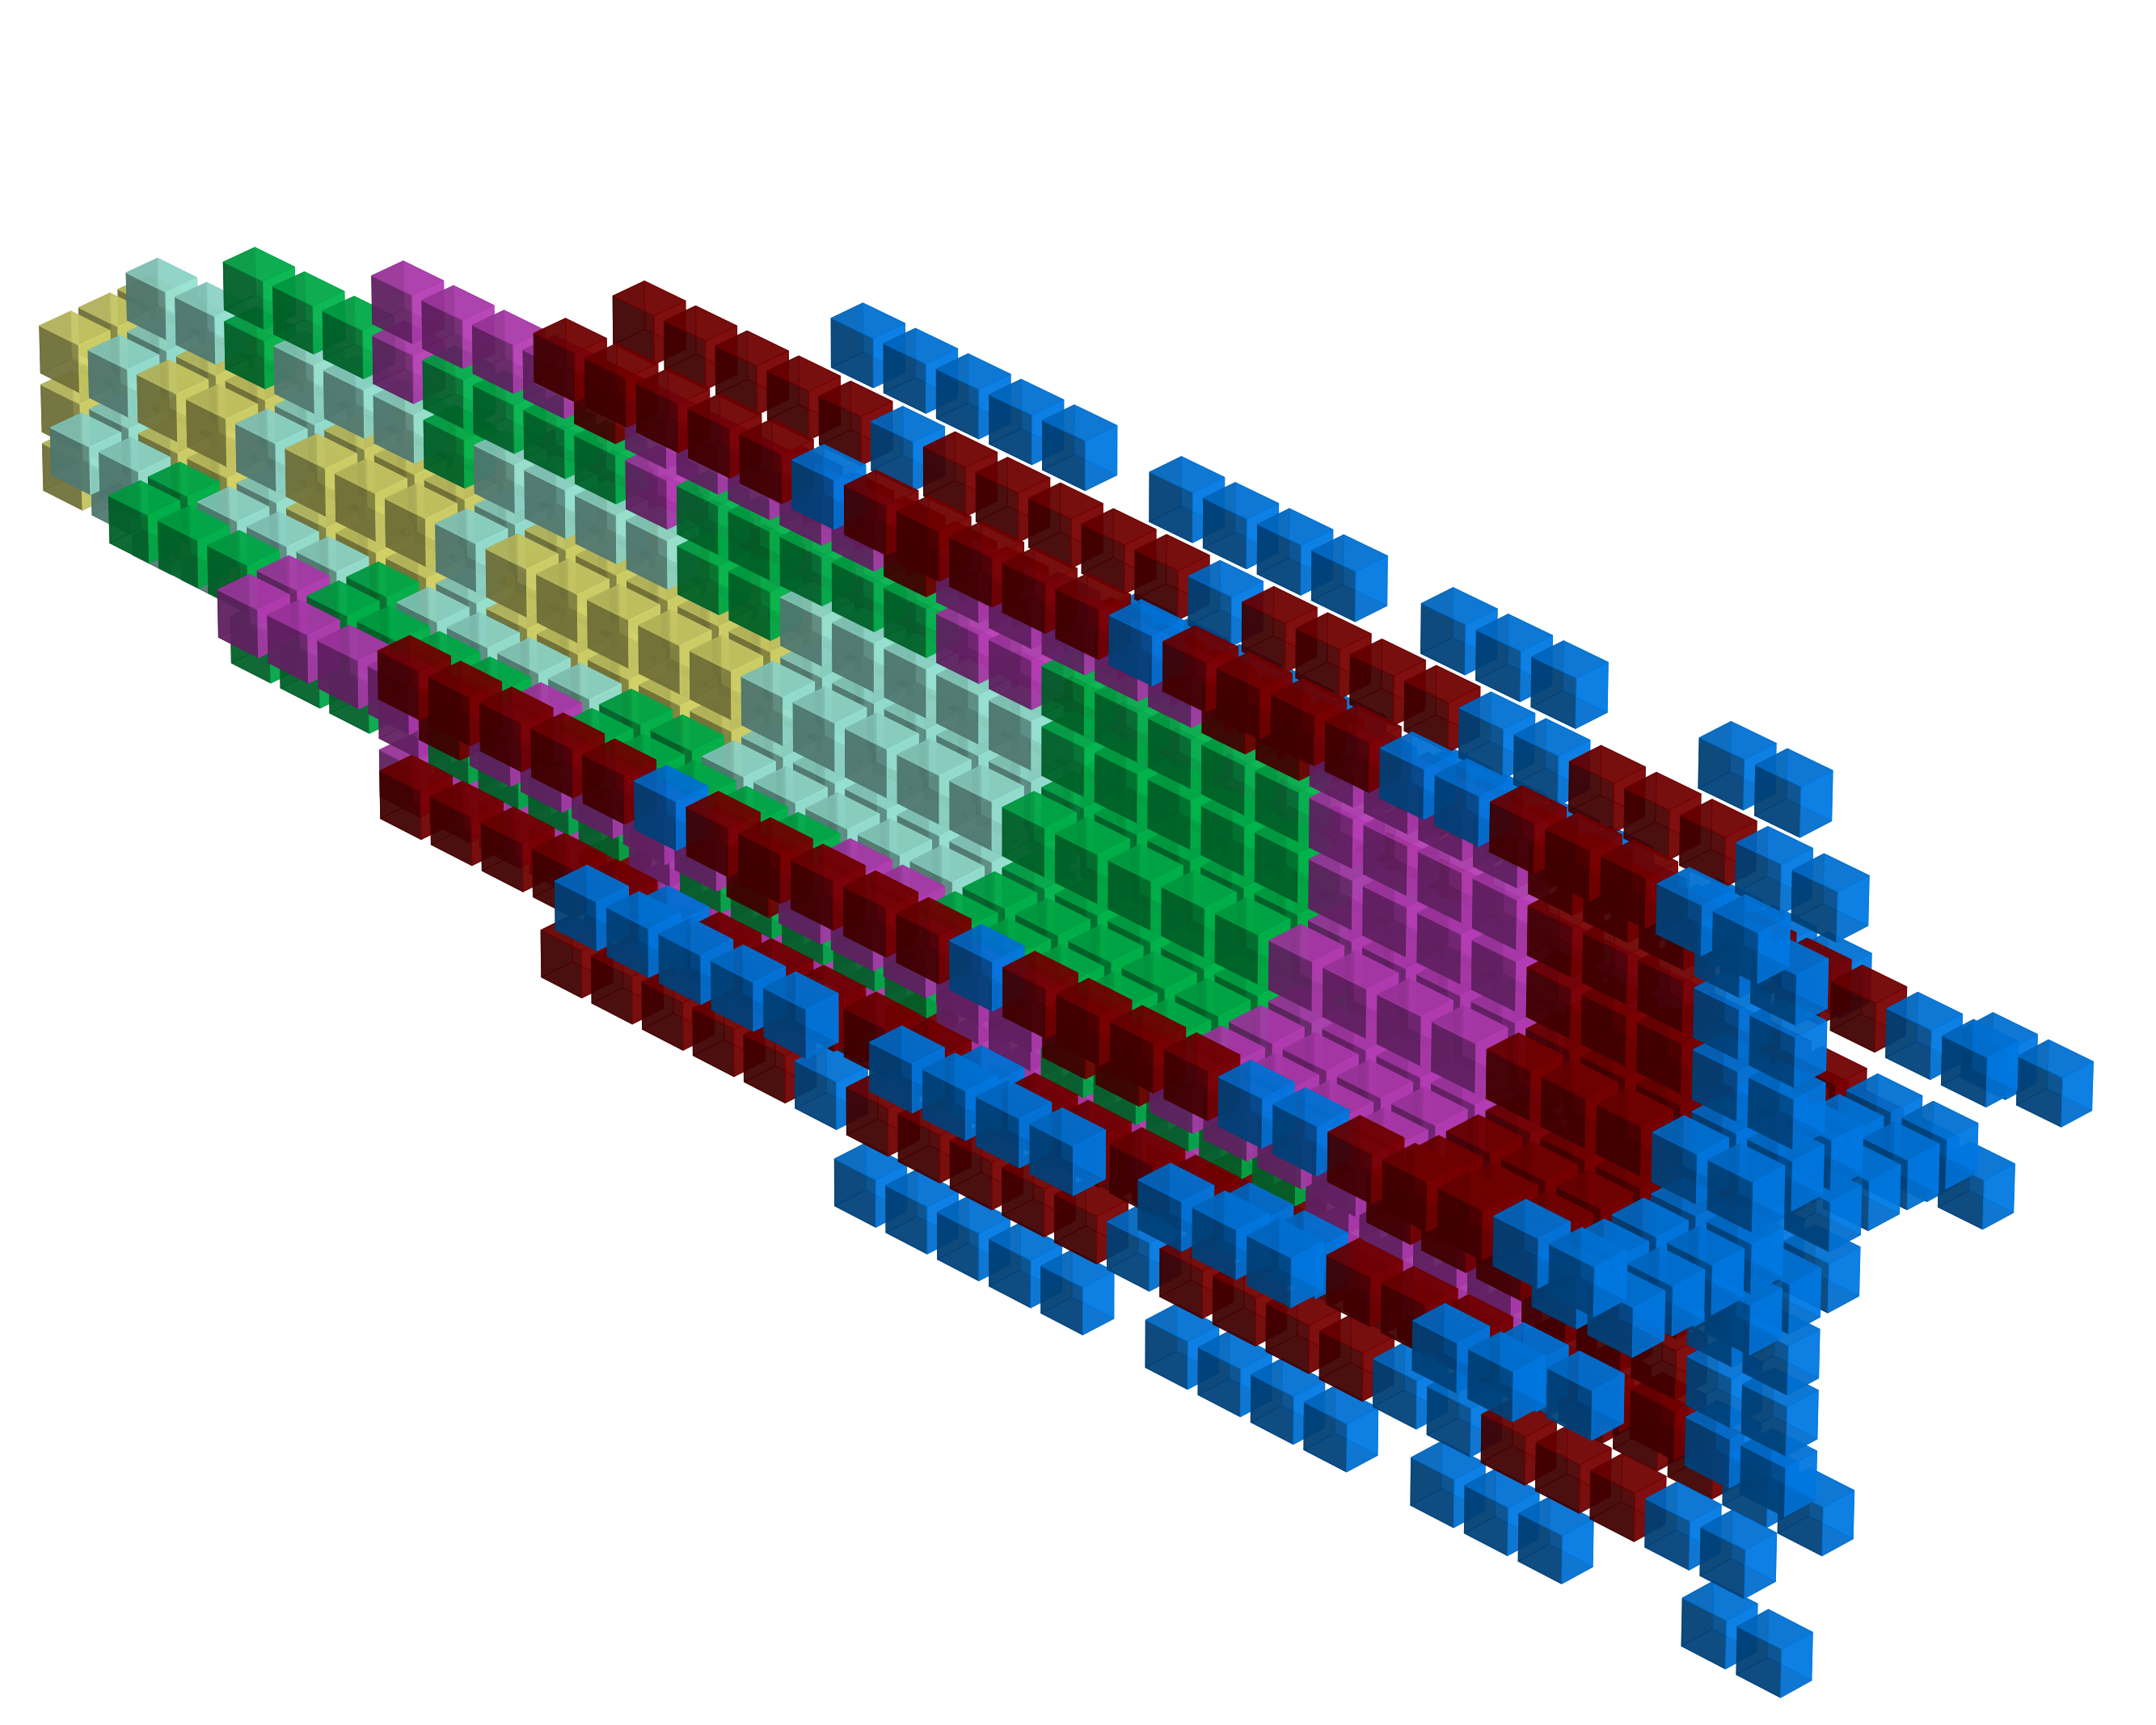
\includegraphics[width=12cm]{src/patterns/pattern0-45.png}%
    \end{adjustbox}
    \begin{adjustbox}{width=12cm,margin=0cm -2cm}
      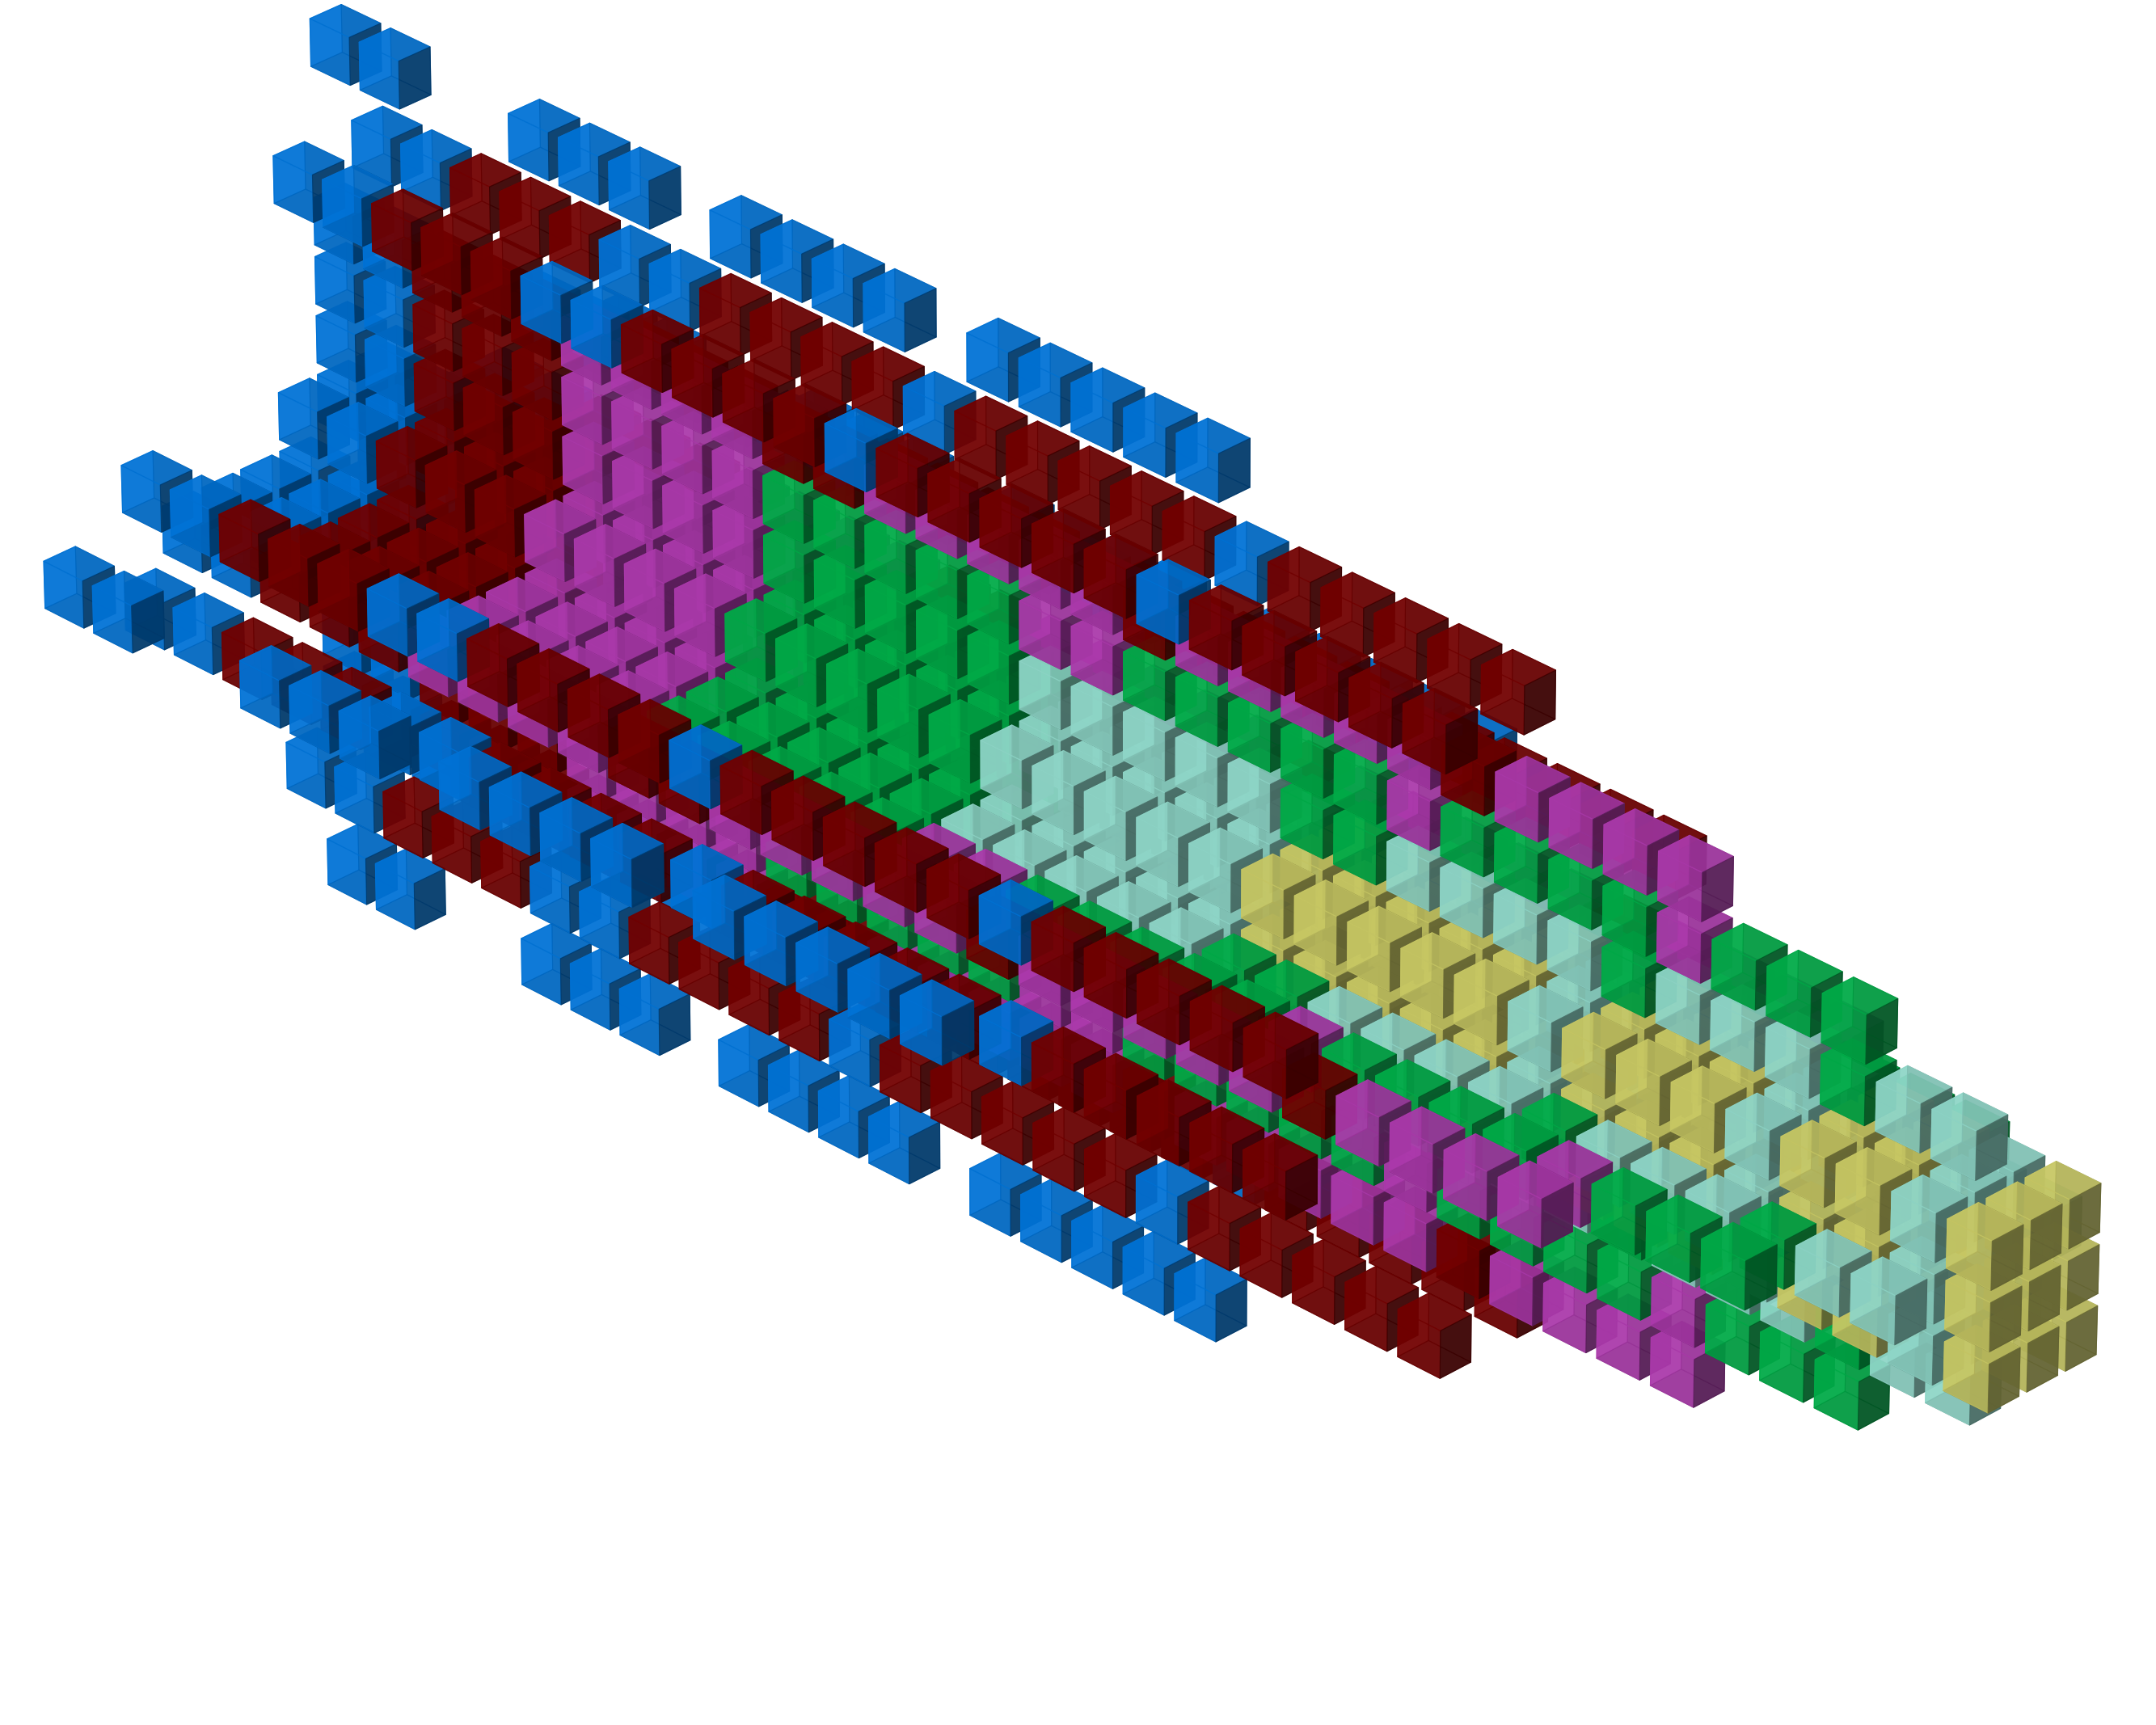
\includegraphics[width=12cm]{src/patterns/pattern0-225.png}%
    \end{adjustbox}
\caption{Evolution of the 'Star One' pattern.}
\end{figure}

\begin{lstlisting}[caption=Source code for the Star.]
starOneXPosArray  
  .BYTE $00,$01,$01,$01,$00,$FF,$FF,$FF,$55       ;        5       
  .BYTE $00,$02,$00,$FE,$55                       ;                
  .BYTE $00,$03,$00,$FD,$55                       ;       4 4      
  .BYTE $00,$04,$00,$FC,$55                       ;        3       
  .BYTE $FF,$01,$05,$05,$01,$FF,$FB,$FB,$55       ;        2       
  .BYTE $00,$07,$00,$F9,$55                       ;        1       
  .BYTE $55                                       ;   4   000   4  
starOneYPosArray                                  ; 5  3210 0123  5  
  .BYTE $FF,$FF,$00,$01,$01,$01,$00,$FF,$55       ;   4   000   4  
  .BYTE $FE,$00,$02,$00,$55                       ;        1       
  .BYTE $FD,$00,$03,$00,$55                       ;        2       
  .BYTE $FC,$00,$04,$00,$55                       ;        3       
  .BYTE $FB,$FB,$FF,$01,$05,$05,$01,$FF,$55       ;       4 4      
  .BYTE $F9,$00,$07,$00,$55                       ;                
  .BYTE $55                                       ;        5       
\end{lstlisting}

Somehow this data is encoding the pattern that Psychedelia is drawing. It looks to be a list of X and Y 
co-ordinates with the X co-ordinates stored in \icode{starOneXPosArray} and the Y co-ordinates in
\icode{starOneYPosArray}. The only problem is they don't look much like co-ordinates. After puzzling 
for a little while I realized what's going on here. The very first pair of bytes is \icode{\$00} from
\icode{starOneXPosArray} and \icode{\$FF} from \icode{starOneYPosArray}. That can't mean that the X,Y
position is \icode{(0,255)}, so what if \icode{\$FF} means something else? What about \icode{-1}? That
would mean \icode{\$FE} means \icode{-2} and so on. Now things start to make sense. If we treat 'C' as our origin the first line of 
each array actually contains a unit distance plot around the origin. We can represent it with \icode{0s} around the origin as follows:

\begin{lstlisting}
                           000      
                           0C0        
                           000      
\end{lstlisting}

Putting our rudimentary diagram side by side with our data arrays we have:
\begin{lstlisting}
starOneXPosArray  
  .BYTE $00,$01,$01,$01,$00,$FF,$FF,$FF,$55       ;       000      
starOneYPosArray                                  ;       0C0        
  .BYTE $FF,$FF,$00,$01,$01,$01,$00,$FF,$55       ;       000      
\end{lstlisting}

The \icode{\$55} at the end of each line looks like a kind of line-break splitting up the array, so we don't use it for
co-ordinates. 
When we add in the second line from each array, plotting the positions with a \icode{1} this time, we then get:

\begin{lstlisting}[caption=Source code for the Star.]
starOneXPosArray  
  .BYTE $00,$01,$01,$01,$00,$FF,$FF,$FF,$55       ;                
  .BYTE $00,$02,$00,$FE,$55                       ;        1 
                                                  ;       000      
                                                  ;      10 01       
starOneYPosArray                                  ;       000
  .BYTE $FF,$FF,$00,$01,$01,$01,$00,$FF,$55       ;        1  
  .BYTE $FE,$00,$02,$00,$55                       ; 
\end{lstlisting}

And so on, until we build up the picture we found in the inital code above. For some reason the very last 'line' in the 
array is empty, it just contains the delimiter value \icode{\$55}:

\begin{lstlisting}
starOneXPosArray  
  ...
  .BYTE $55  
starOneYPosArray  
  ...
  .BYTE $55      
\end{lstlisting}

It's as though it is just there to make up the numbers, giving us
seven lines of data in total. Let's hold that thought for now.

So we kind of understand an important data structure used
by the code. It seems designed to build the pattern incrementally, one pair of lines from each array at a time.
This matches our intuition of how the painting ought to work given the way we see it operate in use. The pattern isn't drawn
all at once but accumulates on-screen in a way that matches what we're seeing in the way the pattern's co-ordinates
are structured in \icode{starOneXPosArray} and \icode{starOneYPosArray}.

The next thing we might think of looking for is the way the colors are defined. We find them towards the beginning of the file:
\begin{lstlisting}
presetColorValuesArray
  .BYTE BLACK,BLUE,RED,PURPLE,GREEN,CYAN,YELLOW,WHITE
\end{lstlisting}

There are eight colors defined in total, more or less as we suspected. This number is a strange limitation, even for a computer as old
as the Commodore 64 which after all has a total of 16 available. If we look a little closer, the number is even
fewer: the first one listed there is \icode{BLACK} so it doesn't even count as a color. The screen is black already after all, unless we've
painted it with something. Indeed, putting \icode{BLACK} at the 
start like that suggests it is being used to clear a 'pixel' we've already painted. This leaves us with seven 
colours in total. 

So after a brief inspection of just the data we seem to have a system that consists of patterns with seven lines of data and a palette
of seven colors. We would be right to suspect that this is not a coincidence. But we have to dive into the code to see why.

The best place to read code is at the beginning. This doesn't mean from the top of the file but from the place that controls everything
else in the program. In nearly all programs this is the 'main loop', a usually short section of code that runs repeatedly in a loop and
controls the operation of the rest of the program. As it happens, Pyschedelia has two of these! 

The first is what we conventionally 
understand by a 'main loop': the program starts executing this and never stops. It just keeps going around in a circle executing the instructions 
over and over again. Here is a slightly chopped-down picture of Psychedelia's \icode{MainPaintLoop}. We'll see the rest of it later on
but this is enough to help you see how it just goes round-and-round:

\begin{lstlisting}
MainPaintLoop   
  ; Here and elsewhere '...' indicates we've removed some code for brevity.
  ... 
  ; 'X' below is the current index value, the loop increments it at
  ; every iteration and ensures it is always a value between 0 and 31. 
  ; We've cut out the bits that do all that for now to aid clarity.
  ...
  ; Load the value from the current index position in
  ; currentColorIndexArray and store it in colorIndexForCurrentPixel.
  ; The values in currentColorIndexArray array are always between 0 
  ; and 7. 
  LDA currentColorIndexArray,X
  ...
  STA colorIndexForCurrentPixel

  ; Get the X and Y position stored in the current position of each
  ; array.
  LDA pixelXPositionArray,X
  STA pixelXPosition
  LDA pixelYPositionArray,X
  STA pixelYPosition

  ; Where the magic happens.
  JSR PaintStructureAtCurrentPosition

  ; Decrement the value stored in currentColorIndexArray at the
  ; current position, for example from 7 to 6.
  DEC currentColorIndexArray,X

  JMP MainPaintLoop ; And back to the start again!
\end{lstlisting}

What this loop does at every turn is choose a position on the screen and paint the pattern around it. Basically the operation we intuited
when we looked at the \icode{starOneXPosArray} and \icode{starOneYPosArray} data structures above. For this it has a virtual list of
32 positions which it reads from. This list is made up of two actual lists (also known as arrays), one containing the X co-ordinate
of the positions (\icode{pixelXPositionArray}) and one containing the Y co-ordinates (\icode{pixelYPositionArray}). It reads these
from beginning to end and then back to the start again. There's another list it reads from at the same time, \icode{currentColorIndexArray}.
This is also 32 elements long and the values it conatins are always between 0 and 7. The reason for this is that the values
are an index into \icode{presetColorValuesArray}. So
what each value actually tells us is the color that was used as the starting point for painting colors the last time we painted a pattern
using this position in the arrays. For example a value of 5 would indicate \icode{CYAN} since counting from zero bring us to that element
in the list.

\begin{lstlisting}
presetColorValuesArray
  ;       0      1    2     3       4      5     6      7
  .BYTE BLACK, BLUE, RED, PURPLE, GREEN, CYAN, YELLOW, WHITE
\end{lstlisting}

So we have three main arrays in use here. Two giving us a list of positions on the screen (\icode{pixelXPositionArray}, \icode{pixelYPositionArray})
and one giving us a list of colors (\icode{currentColorIndexArray}). I've indicated in the listing above that the magic happens in 
\icode{PaintStructureAtCurrentPosition}. This is where the values retrieved from each of the three lists are put to magical use and colourful things
are drawn on the screen.

\begin{lstlisting}[caption=The arrays have a larger capacity than is actually used\, each one above is 64 bytes long.]
pixelXPositionArray   
  .BYTE $0F,$0E,$0D,$0C,$0B,$0A,$09,$04
  .BYTE $05,$06,$07,$08,$09,$0A,$0B,$0C
  .BYTE $0D,$0E,$0F,$10,$11,$12,$13,$14
  .BYTE $15,$16,$17,$14,$13,$12,$11,$10
  .BYTE $00,$00,$00,$00,$00,$00,$00,$00
  .BYTE $00,$00,$00,$00,$00,$00,$00,$00
  .BYTE $00,$00,$00,$00,$00,$00,$00,$00
  .BYTE $00,$00,$00,$00,$00,$00,$00,$00
pixelYPositionArray   
  .BYTE $0C,$0D,$0E,$0F,$0F,$0F,$0E,$04
  .BYTE $04,$04,$04,$04,$04,$04,$04,$05
  .BYTE $06,$07,$08,$09,$0A,$0B,$0C,$0D
  .BYTE $0D,$0D,$0D,$07,$09,$09,$0A,$0B
  .BYTE $00,$00,$00,$00,$00,$00,$00,$00
  .BYTE $00,$00,$00,$00,$00,$00,$00,$00
  .BYTE $00,$00,$00,$00,$00,$00,$00,$00
  .BYTE $00,$00,$00,$00,$00,$00,$00,$00
currentColorIndexArray   
  .BYTE $FF,$FF,$FF,$FF,$FF,$FF,$FF,$FF
  .BYTE $FF,$FF,$FF,$FF,$FF,$FF,$FF,$FF
  .BYTE $FF,$FF,$FF,$FF,$FF,$FF,$FF,$FF
  .BYTE $FF,$FF,$FF,$FF,$FF,$FF,$FF,$FF
  .BYTE $00,$00,$00,$00,$00,$00,$00,$00
  .BYTE $00,$00,$00,$00,$00,$00,$00,$00
  .BYTE $00,$00,$00,$00,$00,$00,$00,$00
  .BYTE $00,$00,$00,$00,$00,$00,$00,$00
\end{lstlisting}

Before we delve into how \icode{PaintStructureAtCurrentPosition} achieves this, we should answer a question that might be occuring to you: how
are the three lists above populated? There's no sign of anything happening to them in \icode{MainPaintLoop}. It just reads them over and
over again forever. The answer to this lies in the program's second 'main loop' that we mentioned earlier. 
Strictly speaking it's not a loop at all but what is known
as a 'hardware interrupt'. A hardware interrupt is when a computer wakes up periodically (usually many times every second!) and executes
some code. This is useful because programmers can nominate some code for it to run each time and as a bonus specify exactly when the code
should run, for example just after the screen has been painted or even at a specific point during the painting of the screen.  

Psychedelia doesn't get too fancy in this regard. The code it nominates is specified to run once per screen paint. This code concerns itself
with one thing: collecting the user's key presses and most importantly from our point of view the key presses that move the cursor around
the screen. This is the stuff that feeds our \icode{pixelXPositionArray} and \icode{pixelYPositionArray}.

\begin{lstlisting}
MainInterruptHandler   
  ...
  ; Increment our index.
  INC indexIntoArrays
  LDA indexIntoArrays
  ; Ensure indexIntoArrays loops back to zero once
  ; if reaches MAX_INDEX_VALUE (i.e. 31).
  AND MAX_INDEX_VALUE
  STA indexIntoArrays
  ...
  ; With an update counter stored in the 'A' register,
  ; move it to 'X' so we can use it below.
  TAX
  ...
  ; Feed our three beasts!
  LDA cursorXPosition
  STA pixelXPositionArray,X
  LDA cursorYPosition
  STA pixelYPositionArray,X
  LDA #COLOR_MAX                ; COLOR_MAX = 7
  STA currentColorIndexArray,X

  JMP RETURN_FROM_INTERRUPT
\end{lstlisting}

As you can see in the last few lines above we periodically feed the cursor position into \icode{pixelXPositionArray} and \icode{pixelYPositionArray}.
We also feed a 7 (\icode{COLOR\_MAX}) into the \icode{currentColorIndexArray}. So if we stay absolutely still and don't move the cursor at all, after
a short while the three arrays will end up looking like this. With \icode{\$1E} (30) as the X position in each slot and \icode{\$0D} (13) as the Y
position in each slot.

\begin{lstlisting}
pixelXPositionArray   
  .BYTE $1E,$1E,$1E,$1E,$1E,$1E,$1E,$1E
  .BYTE $1E,$1E,$1E,$1E,$1E,$1E,$1E,$1E
  .BYTE $1E,$1E,$1E,$1E,$1E,$1E,$1E,$1E
  .BYTE $1E,$1E,$1E,$1E,$1E,$1E,$1E,$1E
  ...
pixelYPositionArray   
  .BYTE $0D,$0D,$0D,$0D,$0D,$0D,$0D,$0D
  .BYTE $0D,$0D,$0D,$0D,$0D,$0D,$0D,$0D
  .BYTE $0D,$0D,$0D,$0D,$0D,$0D,$0D,$0D
  .BYTE $0D,$0D,$0D,$0D,$0D,$0D,$0D,$0D
  ...
currentColorIndexArray   
  .BYTE $07,$07,$07,$07,$07,$07,$07,$07
  .BYTE $07,$07,$07,$07,$07,$07,$07,$07
  .BYTE $07,$07,$07,$07,$07,$07,$07,$07
  .BYTE $07,$07,$07,$07,$07,$07,$07,$07
  ...
\end{lstlisting}

Armed with an understanding of the data that is feeding into the pixel generation of Psychedelia we can now move on to getting our
heads around the code that implements the pixel generation itself. This starts in the routine that reads in the pattern's data
structure, \icode{PaintStructureAtCurrentPosition}, called from our main loop every time we read in from our three arrays above.



Remember that our data structure has seven lines in it, each delimited by a \icode{\$55} at its end. This routine will read and
paint a number of these lines. The number is determined by the value we read from \icode{currentColorIndexArray} and stored in
\icode{currentValueInColorIndexArray}. For example if we read \icode{6} it will only paint the first line from each of 
\icode{starOneXPosArray} and \icode{starOneYPosArray} (2 lines in total):

\begin{figure}[H]
  {
    \setlength{\tabcolsep}{3.0pt}
    \setlength\cmidrulewidth{\heavyrulewidth} % Make cmidrule = 
    \begin{adjustbox}{height=1cm,center}
      \footnotesize
      \begin{tabular}{ll}

        \makecell[l]{
          \icode{.BYTE \$00,\$01,\$01,\$01,\$00,\$FF,\$FF,\$FF,\$55}\\
          \icode{.BYTE \$FF,\$FF,\$00,\$01,\$01,\$01,\$00,\$FF,\$55}
        } & \makecell[l]{
          
\includegraphics[width=1.3cm]{src/patterns/pixels/pixel_pattern0_0.png}%
        } \\
        \midrule
      \end{tabular}
    \end{adjustbox}
  }
\end{figure}

If we read \icode{5} it will only paint the first 2 lines of each array (4 lines in total).

\begin{figure}[H]
  {
    \setlength{\tabcolsep}{3.0pt}
    \setlength\cmidrulewidth{\heavyrulewidth} % Make cmidrule = 
    \begin{adjustbox}{height=2cm,center}
      \footnotesize
      \begin{tabular}{ll}

        \makecell[l]{
          \icode{.BYTE \$00,\$01,\$01,\$01,\$00,\$FF,\$FF,\$FF,\$55}\\
          \icode{.BYTE \$FF,\$FF,\$00,\$01,\$01,\$01,\$00,\$FF,\$55}
        } & \makecell[l]{
          
\includegraphics[width=1.3cm]{src/patterns/pixels/pixel_pattern0_0.png}%
        } \\
        \midrule
        \makecell[l]{
          \icode{.BYTE \$00,\$02,\$00,\$FE}\\
          \icode{.BYTE \$FE,\$00,\$02,\$00}
        } & \makecell[l]{
          
\includegraphics[width=1.3cm]{src/patterns/pixels/pixel_pattern0_1.png}%
          
\includegraphics[width=1.3cm]{src/patterns/pixels/pixel_pattern0_2.png}%
        } \\
        \midrule
      \end{tabular}
    \end{adjustbox}
  }
\end{figure}

We can see how this logic is implemented in this heavily abbreviated version of \icode{PaintStructureAtCurrentPosition}.

\begin{lstlisting}
PaintStructureAtCurrentPosition   
  ..
  LDA #NUM_ARRAYS ; NUM_ARRAYS = 7
  STA countToMatchCurrentIndex

  ..
  ; Y starts out at zero here. We use it as an index
  ; for reading in starOneXPosArray and starOneYPosArray
  ; one byte at a time.
LineReadLoop   
  LDA initialPixelXPosition
  CLC 
  ADC starOneXPosArray,Y
  STA pixelXPosition

  LDA initialPixelYPosition
  CLC 
  ADC starOneYPosArray,Y
  STA pixelYPosition
  ...
  JSR PaintPixelForCurrentSymmetry
  ...
  INY 

  ; Loop if we haven't reached the end of the current
  ; line in starOneXPosArray
  LDA starOneXPosArray,Y
  CMP #$55
  BNE LineReadLoop

  ; Check if we've reached the last line in the structure
  ; for this visit. This will always be one more than our 
  ; last visit.
  DEC countToMatchCurrentIndex
  LDA countToMatchCurrentIndex
  CMP currentValueInColorIndexArray
  BEQ Return
  CMP #$01
  BEQ Return

  ; Move to the start of the next line in starOneXPosArray/
  ; starOneYPosArray.
  INY 
  JMP LineReadLoop

Return   
  ...
  RTS 
\end{lstlisting}

It initializes \icode{countToMatchCurrentIndex} to 7:
\begin{lstlisting}
  LDA #NUM_ARRAYS ; NUM_ARRAYS = 7
  STA countToMatchCurrentIndex
\end{lstlisting}

and decrements this value after reading each line 
\begin{lstlisting}
  DEC countToMatchCurrentIndex
\end{lstlisting}

until it matches the value in \icode{currentValueInColorIndexArray} or we have reached the last line in the structure.

\begin{lstlisting}
  LDA countToMatchCurrentIndex
  CMP currentValueInColorIndexArray
  BEQ Return
  CMP #$01
  BEQ Return
\end{lstlisting}

We can see how this works in practice with a few examples. In our very first visit to \icode{PaintStructureAtCurrentPosition}
we have a value of \icode{\$06} in \icode{currentValueInColorIndexArray}. So we paint one phase from \icode{starOneX/YPosArray}:

\begin{figure}[H]                                                              
  {                                                                            
    \setlength{\tabcolsep}{3.0pt}                                              
    \setlength\cmidrulewidth{\heavyrulewidth} % Make cmidrule =                
    \begin{adjustbox}{width=7cm,center}                                       
      \footnotesize                                                            
      \begin{tabular}{ll}
				\makecell[l]{                                                          
				\icode{currentColorIndexArray} Bytes 26-32:\\
				\icode{.BYTE  \$FF,\$FF,\textcolor{red}{\$06},\$FF,\$FF,\$FF,\$FF}\\
				} & \makecell[l]{                                                      
				
\includegraphics[width=1.3cm]{src/patterns/maps/pixel_pattern_0.png}%
				} \\                                                                   
      \end{tabular}                                                            
    \end{adjustbox}                                                            
  }                                                                            
\end{figure}                                                                   

The next time we visit \icode{currentValueInColorIndexArray} is \icode{\$05}, so we paint two phases:

\begin{figure}[H]                                                              
  {                                                                            
    \setlength{\tabcolsep}{3.0pt}                                              
    \setlength\cmidrulewidth{\heavyrulewidth} % Make cmidrule =                
    \begin{adjustbox}{width=8cm,center}                                       
      \footnotesize                                                            
      \begin{tabular}{ll}
				\makecell[l]{                                                          
				\icode{currentColorIndexArray} Bytes 26-32:\\
				\icode{.BYTE  \$FF,\$FF,\textcolor{red}{\$05},\$07,\$FF,\$FF,\$FF}\\
				} & \makecell[l]{                                                      
				
\includegraphics[width=1.3cm]{src/patterns/maps/pixel_pattern_1.png}%
				
\includegraphics[width=1.3cm]{src/patterns/maps/pixel_pattern_2.png}%
				} \\                                                                   
      \end{tabular}                                                            
    \end{adjustbox}                                                            
  }                                                                            
\end{figure}                                                                   

Notice that the value of \icode{\$05} determines two things: that we paint two phases of the overall pattern and the color
we paint them is \icode{CYAN} (because \icode{05} points to \icode{CYAN} in \icode{presetColorValuesArray}). We'll see
how this is done shortly.

In yet another example for later on in the pattern's evolution we can see this:

\begin{figure}[H]                                                              
  {                                                                            
    \setlength{\tabcolsep}{3.0pt}                                              
    \setlength\cmidrulewidth{\heavyrulewidth} % Make cmidrule =                
    \begin{adjustbox}{width=10cm,center}                                       
      \footnotesize                                                            
      \begin{tabular}{ll}
				\makecell[l]{                                                          
				\icode{currentColorIndexArray} Bytes 26-32:\\
				\icode{.BYTE  \$FF,\$FF,\textcolor{red}{\$03},\$05,\$06,\$FF,\$FF}\\
				} & \makecell[l]{                                                      
				
\includegraphics[width=1.3cm]{src/patterns/maps/pixel_pattern_7.png}%
				
\includegraphics[width=1.3cm]{src/patterns/maps/pixel_pattern_8.png}%
				
\includegraphics[width=1.3cm]{src/patterns/maps/pixel_pattern_9.png}%
				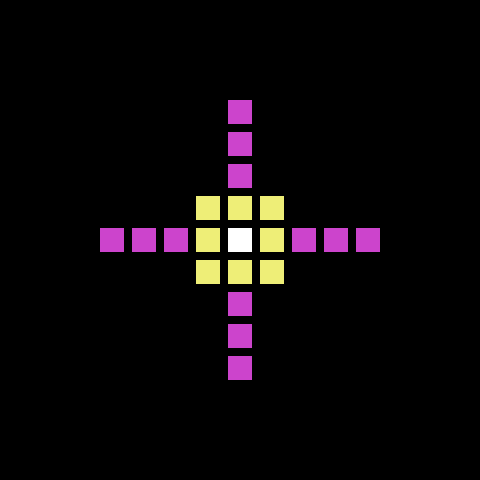
\includegraphics[width=1.3cm]{src/patterns/maps/pixel_pattern_10.png}%
				} \\                                                                   
			\end{tabular}                                                            
    \end{adjustbox}                                                            
  }                                                                            
\end{figure}                                                                   

Here \icode{\$03} points to \icode{PURPLE} in \icode{presetColorValuesArray} so each phase is painted in purple. And again
because \icode{currentValueInColorIndexArray} is \icode{\$03} we paint four phases (7 - 3 = 4). For some reason though, we
didn't paint any purple in the first phase - notice the pattern has stayed yellow and green.  


To understand why this is so we will have to look into how the actual painting is handled by \icode{PaintPixelForCurrentSymmetry}. This is called for each pair of positions read
in from \icode{starOneXPosArray} and \icode{starOneYPosArray} and stored in \icode{pixelXPosition} and \icode{pixelYPosition}.
In its simplest use \icode{PaintPixelForCurrentSymmetry} just ends up calling another routine \icode{PaintPixel} directly.
That's the use we'll look at here, so we can skip straight to \icode{PaintPixel} instead.

As we saw above like \icode{PaintStructureAtCurrentPosition}
its behaviour is controlled by \icode{currentValueInColorIndexArray}. But whereas there it was used to control how many
stages of the structure to paint, here it is used to figure out which color to paint the pixel or whether to paint the pixel 
at all.

The core of this operation lies as you might imagine in seeing what color the pixel is already. The first step of this involves
using the \icode{pixelXPosition} and \icode{pixelYPosition} to load the color information for the position on screen we might 
want to paint: 

\begin{lstlisting}
PaintPixel   
  ...
  JSR LoadXAndYPosition
  ; Y now contains the pixelXPosition
  LDA (currentLineForPixelInColorRamLoPtr),Y
  ; Make sure the color we get is addressable by
  ; presetColorValuesArray.
  AND #COLOR_MAX
\end{lstlisting}

Now while this value will be between 0 and 7, representing one of the seven colors we paint with, it isn't one we can directly
compare with \icode{currentValueInColorIndexArray}. This is because \icode{currentValueInColorIndexArray} is an index rather
than a color value. So what we need to do with the color we've retrieved from the screen is figure out what index in 
\icode{presetColorValuesArray} is refers to:

\begin{lstlisting}
presetColorValuesArray
  ;       0      1    2     3       4      5     6      7
  .BYTE BLACK, BLUE, RED, PURPLE, GREEN, CYAN, YELLOW, WHITE

PaintPixel   
  ...
  ; Translate the color at the current pixel to an
  ; index value so that it can be compared with
  ; currentValueInColorIndexArray
  LDX #$00
FindIndexLoop
  CMP presetColorValuesArray,X
  BEQ b4096
  INX 
  CPX #COLOR_MAX + 1
  BNE FindIndexLoop
\end{lstlisting}

The snippet of code above is what does this. For example where it retrieves the color \icode{PURPLE} from the position on screen
it converts it to a value of \icode{3} (the index position of \icode{PURPLE} in \icode{presetColorValuesArray}).

Once we have that we can now decide whether or not to paint the pixel with the color referenced by \icode{currentValueInColorIndexArray}.
What decides this for us is whether the current color at the position in the screen is any of:
\begin{itemize}
  \item black, i.e. nothing has been painted there yet;
  \item the same as the color we want to paint;
  \item or the one just above it in \icode{presetColorValuesArray}.
\end{itemize}

So if the color we want to paint is \icode{PURPLE}, we will only paint on black cells, purple cells, or green cells. Reminding ourselves
again that \icode{GREEN} appears after \icode{PURPLE} in \icode{presetColorValuesArray}.

\begin{lstlisting}
presetColorValuesArray
  ;       0      1    2     3       4      5     6      7
  .BYTE BLACK, BLUE, RED, PURPLE, GREEN, CYAN, YELLOW, WHITE
\end{lstlisting}

This explains what we saw a little earlier. When painting purple we didn't paint anything in the first phase because the cells at that position
were yellow. However in the phases after that we could paint over the green and black cells.

\begin{figure}[H]                                                              
  {                                                                            
    \setlength{\tabcolsep}{3.0pt}                                              
    \setlength\cmidrulewidth{\heavyrulewidth} % Make cmidrule =                
    \begin{adjustbox}{width=10cm,center}                                       
      \footnotesize                                                            
      \begin{tabular}{ll}
				\makecell[l]{                                                      
				
\includegraphics[width=1.3cm]{src/patterns/maps/pixel_pattern_7.png}%
				
\includegraphics[width=1.3cm]{src/patterns/maps/pixel_pattern_8.png}%
				
\includegraphics[width=1.3cm]{src/patterns/maps/pixel_pattern_9.png}%
				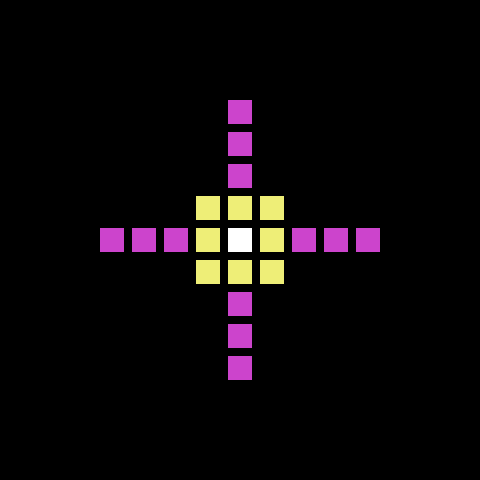
\includegraphics[width=1.3cm]{src/patterns/maps/pixel_pattern_10.png}%
				} \\                                                                   
			\end{tabular}                                                            
    \end{adjustbox}                                                            
  }                                                                            
\caption{Painting only green and black cells, ignoring yellow.}
\end{figure}                                                                   

% Generated with Pattern 0 Evolution - Tracking Array States.ipynb
\begin{figure}[H]
  {
    \setlength{\tabcolsep}{3.0pt}
    \setlength\cmidrulewidth{\heavyrulewidth} % Make cmidrule = 
    \begin{adjustbox}{width=13cm,center}
      \footnotesize
      \begin{tabular}{rl}
        \makecell[l]{
          \subfile{patterns/maps/pattern0_ram_stage7.tex}
          \subfile{patterns/maps/pattern0_ram_stage8.tex}
          \subfile{patterns/maps/pattern0_ram_stage9.tex}
          \subfile{patterns/maps/pattern0_ram_stage10.tex}
        }\\
      \end{tabular}
    \end{adjustbox}
  }
\caption{The same as above but this time with the index values for each cell. We can only paint in a cell that is black, the same
  color as the one we want to paint, or just below it in \icode{presetColorValuesArray}.}
\end{figure}
In practice this means checking whether the color referenced by \icode{current\-ValueInColorIndexArray} is less than or equal 
to the one we want to paint (\icode{indexOfCurrentColor}). In \icode{CheckIf\-ShouldPaintPixel} we implement this check:

\begin{lstlisting}
PaintPixel   
  ...
  ; If the color value at the current pixel (indexOfCurrentColor)
  ; is the one 'after' the new one in presetColorValuesArray
  ; (currentValueInColorIndexArray) then we paint it,
  ; otherwise we ignore it.
CheckIfShouldPaintPixel
  TXA 
  STA indexOfCurrentColor
  LDX currentValueInColorIndexArray
  INX 
  CPX indexOfCurrentColor
  BEQ ActuallyPaintPixel
  BPL ActuallyPaintPixel
  RTS 

ActuallyPaintPixel   
  LDX currentValueInColorIndexArray
  LDA presetColorValuesArray,X
  STA (currentLineForPixelInColorRamLoPtr),Y
  RTS 

\end{lstlisting}

We do it by first loading \icode{currentValueInColorIndexArray} to the  \icode{X} register:
\begin{lstlisting}
  LDX currentValueInColorIndexArray
\end{lstlisting}

Then incrementing it:
\begin{lstlisting}
  INX 
\end{lstlisting}

Then seeing if our current colour is equal to (\icode{BEQ}) or greater (\icode{BPL}) than it:
\begin{lstlisting}
  LDX currentValueInColorIndexArray
  CPX indexOfCurrentColor
  BEQ ActuallyPaintPixel
  BPL ActuallyPaintPixel
\end{lstlisting}

If either of these hold we can actually paint the pixel:
\begin{lstlisting}
  LDX currentValueInColorIndexArray
  LDA presetColorValuesArray,X
  STA (currentLineForPixelInColorRamLoPtr),Y
  RTS 
\end{lstlisting}

How, you might wonder, do any of those four lines actually paint a pixel? For that, we will have to 
look at the code in a little more detail and explain the mechanics of the C64 screen painting mechanism
while we're at it. This we will do in the next chapter. But for now, here are the fruits of \icode{PaintPixel}
when running through the full sequence of painting a star-shaped thing following the algorithm we've 
just described.

\begin{figure}[H]
    \centering
    \foreach \l in {0, 1, ..., 134}
    {
      \begin{subfigure}{0.1\textwidth}
      \includegraphics[width=1cm]{patterns/maps/pixel_pattern_\l.png}%
      \end{subfigure}
    }%
\caption{The full standard sequence of a star-shaped thing.}
\end{figure}
\clearpage





